%%%%%%%%%%%%%%%%%%%%%%%%%%%%%%%%%%%%%%%%%
% Short Three-Column Newsletter
% LaTeX Template
% Version 1.0 (11/9/13)
%
% Original author:
% Frits Wenneker (http://www.howtotex.com) 
% With extensive modifications by:
% Vel (vel@latextemplates.com)
% 
% This template has been downloaded from:
% http://www.LaTeXTemplates.com
%
% License:
% CC BY-NC-SA 3.0 (http://creativecommons.org/licenses/by-nc-sa/3.0/)
%
%%%%%%%%%%%%%%%%%%%%%%%%%%%%%%%%%%%%%%%%%

%----------------------------------------------------------------------------------------
%	PACKAGES AND DOCUMENT CONFIGURATIONS
%----------------------------------------------------------------------------------------

\documentclass[10pt,a4paper]{article} % Paper type (a4paper, usletter or legal) and font size (10, 11 or 12)

\setlength\topmargin{-48pt} % Top margin
\setlength\headheight{0pt} % Header height
\setlength\textwidth{7.0in} % Text width
\setlength\textheight{9.5in} % Text height
\setlength\oddsidemargin{-30pt} % Left margin
\setlength\evensidemargin{-30pt} % Left margin (even pages) - only relevant with 'twoside' article option

\usepackage{charter} % Charter font for main content

\frenchspacing % Reduces space after periods to make text more compact for a three-column layout

\usepackage{graphicx} % Required for including images
\usepackage{amssymb,amsmath} % Math packages
\usepackage{multicol} % Required for the three-column layout of the document
\usepackage{url} % Clickable links
\usepackage{enumitem} % Reduces the amount of space within and between lists with [noitemsep,nolistsep]
\usepackage{marvosym} % Required for the use of symbols
\usepackage{wrapfig} % Allows wrapping text around figures
\usepackage[T1]{fontenc} % Use 8-bit encoding that has 256 glyphs
\usepackage{datetime} % Required for defining a custom date style
\newdateformat{mydate}{\monthname[\THEMONTH] \THEYEAR} % Set a custom date format
\usepackage[pdfpagemode=FullScreen, colorlinks=false]{hyperref} % Link colors and PDF behavior in Acrobat
\usepackage{fancyhdr} % Required to define custom headers/footers
\pagestyle{fancy} % Enables the custom headers/footers for all pages following this

%-----------------------------------------------------------
% Header and footer
\lfoot{\footnotesize % Left footer containing newsletter contact information
	The North Venice -- An story based on author's experience\\
	\Mundus\ \href{https://github.com/stefanos1316/my_blog/index.com}{my\_blog/index.com} \quad
	%\Telefon\ Not available yet \quad
	\Letter\ \href{mailto:sgeorgiou@aueb.gr}{sgeorgiou@aueb.gr}
}


\cfoot{} % Empty center footer

\rfoot{\footnotesize ~\\ Page \thepage} % Right footer - page counter

\renewcommand{\headrulewidth}{0.0pt} % No horizontal rule for the header
\renewcommand{\footrulewidth}{0.4pt} % Horizontal rule separating the footer from the document
%-----------------------------------------------------------

%-----------------------------------------------------------
% Define separators
\newcommand{\HorRule}[1]{\noindent\rule{\linewidth}{#1}} % Creates a horizontal rule
\newcommand{\SepRule}{\noindent	% Creates a shorter separator rule
\begin{center}
\rule{250pt}{1pt} % Page width and rule width
\end{center}
}
%-----------------------------------------------------------

%-----------------------------------------------------------
% Define title and article styles
\newcommand{\NewsletterName}[1]{ % Newsletter title
\begin{center}
\Huge \usefont{T1}{fvs}{b}{n} % Use the Bera Sans Bold font
#1
\end{center}	
\par \normalsize \normalfont}

\newcommand{\JournalIssue}[1]{ % Date and issue number at the top of the newsletter
\hfill \textsc{26th of November 2018, No. #1} % Right-aligned date and issue number
\par \normalsize \normalfont}

\newcommand{\NewsItem}[1]{ % News item title
\usefont{T1}{fvs}{n}{n} % Use the Bera Sans Normal font
\vspace{24pt}\large #1\vspace{3pt} % Print the title with space around it in a larger font size
\par \normalsize \normalfont}

\newcommand{\NewsAuthor}[1]{ % Author name under the item title
\hfill by \textsc{#1} \vspace{20pt} % Right-aligned author name in small caps with space after it
\par \normalfont}		

%----------------------------------------------------------------------------------------
%	TITLE
%----------------------------------------------------------------------------------------

\begin{document}

\JournalIssue{1} % Issue number

\NewsletterName{A little long Adventure} % Newsletter title

\noindent\HorRule{3pt} \\[-0.75\baselineskip] % Thick horizontal rule
\HorRule{1pt} % Thin horizontal rule

%----------------------------------------------------------------------------------------
%	MAIN NEWS ITEM
%----------------------------------------------------------------------------------------

\vspace{0.5cm}
\SepRule
\vspace{-0.5cm}

\begin{center}
\begin{minipage}[h]{0.75 \linewidth}
\begin{wrapfigure}{l}{0.45 \textwidth}
	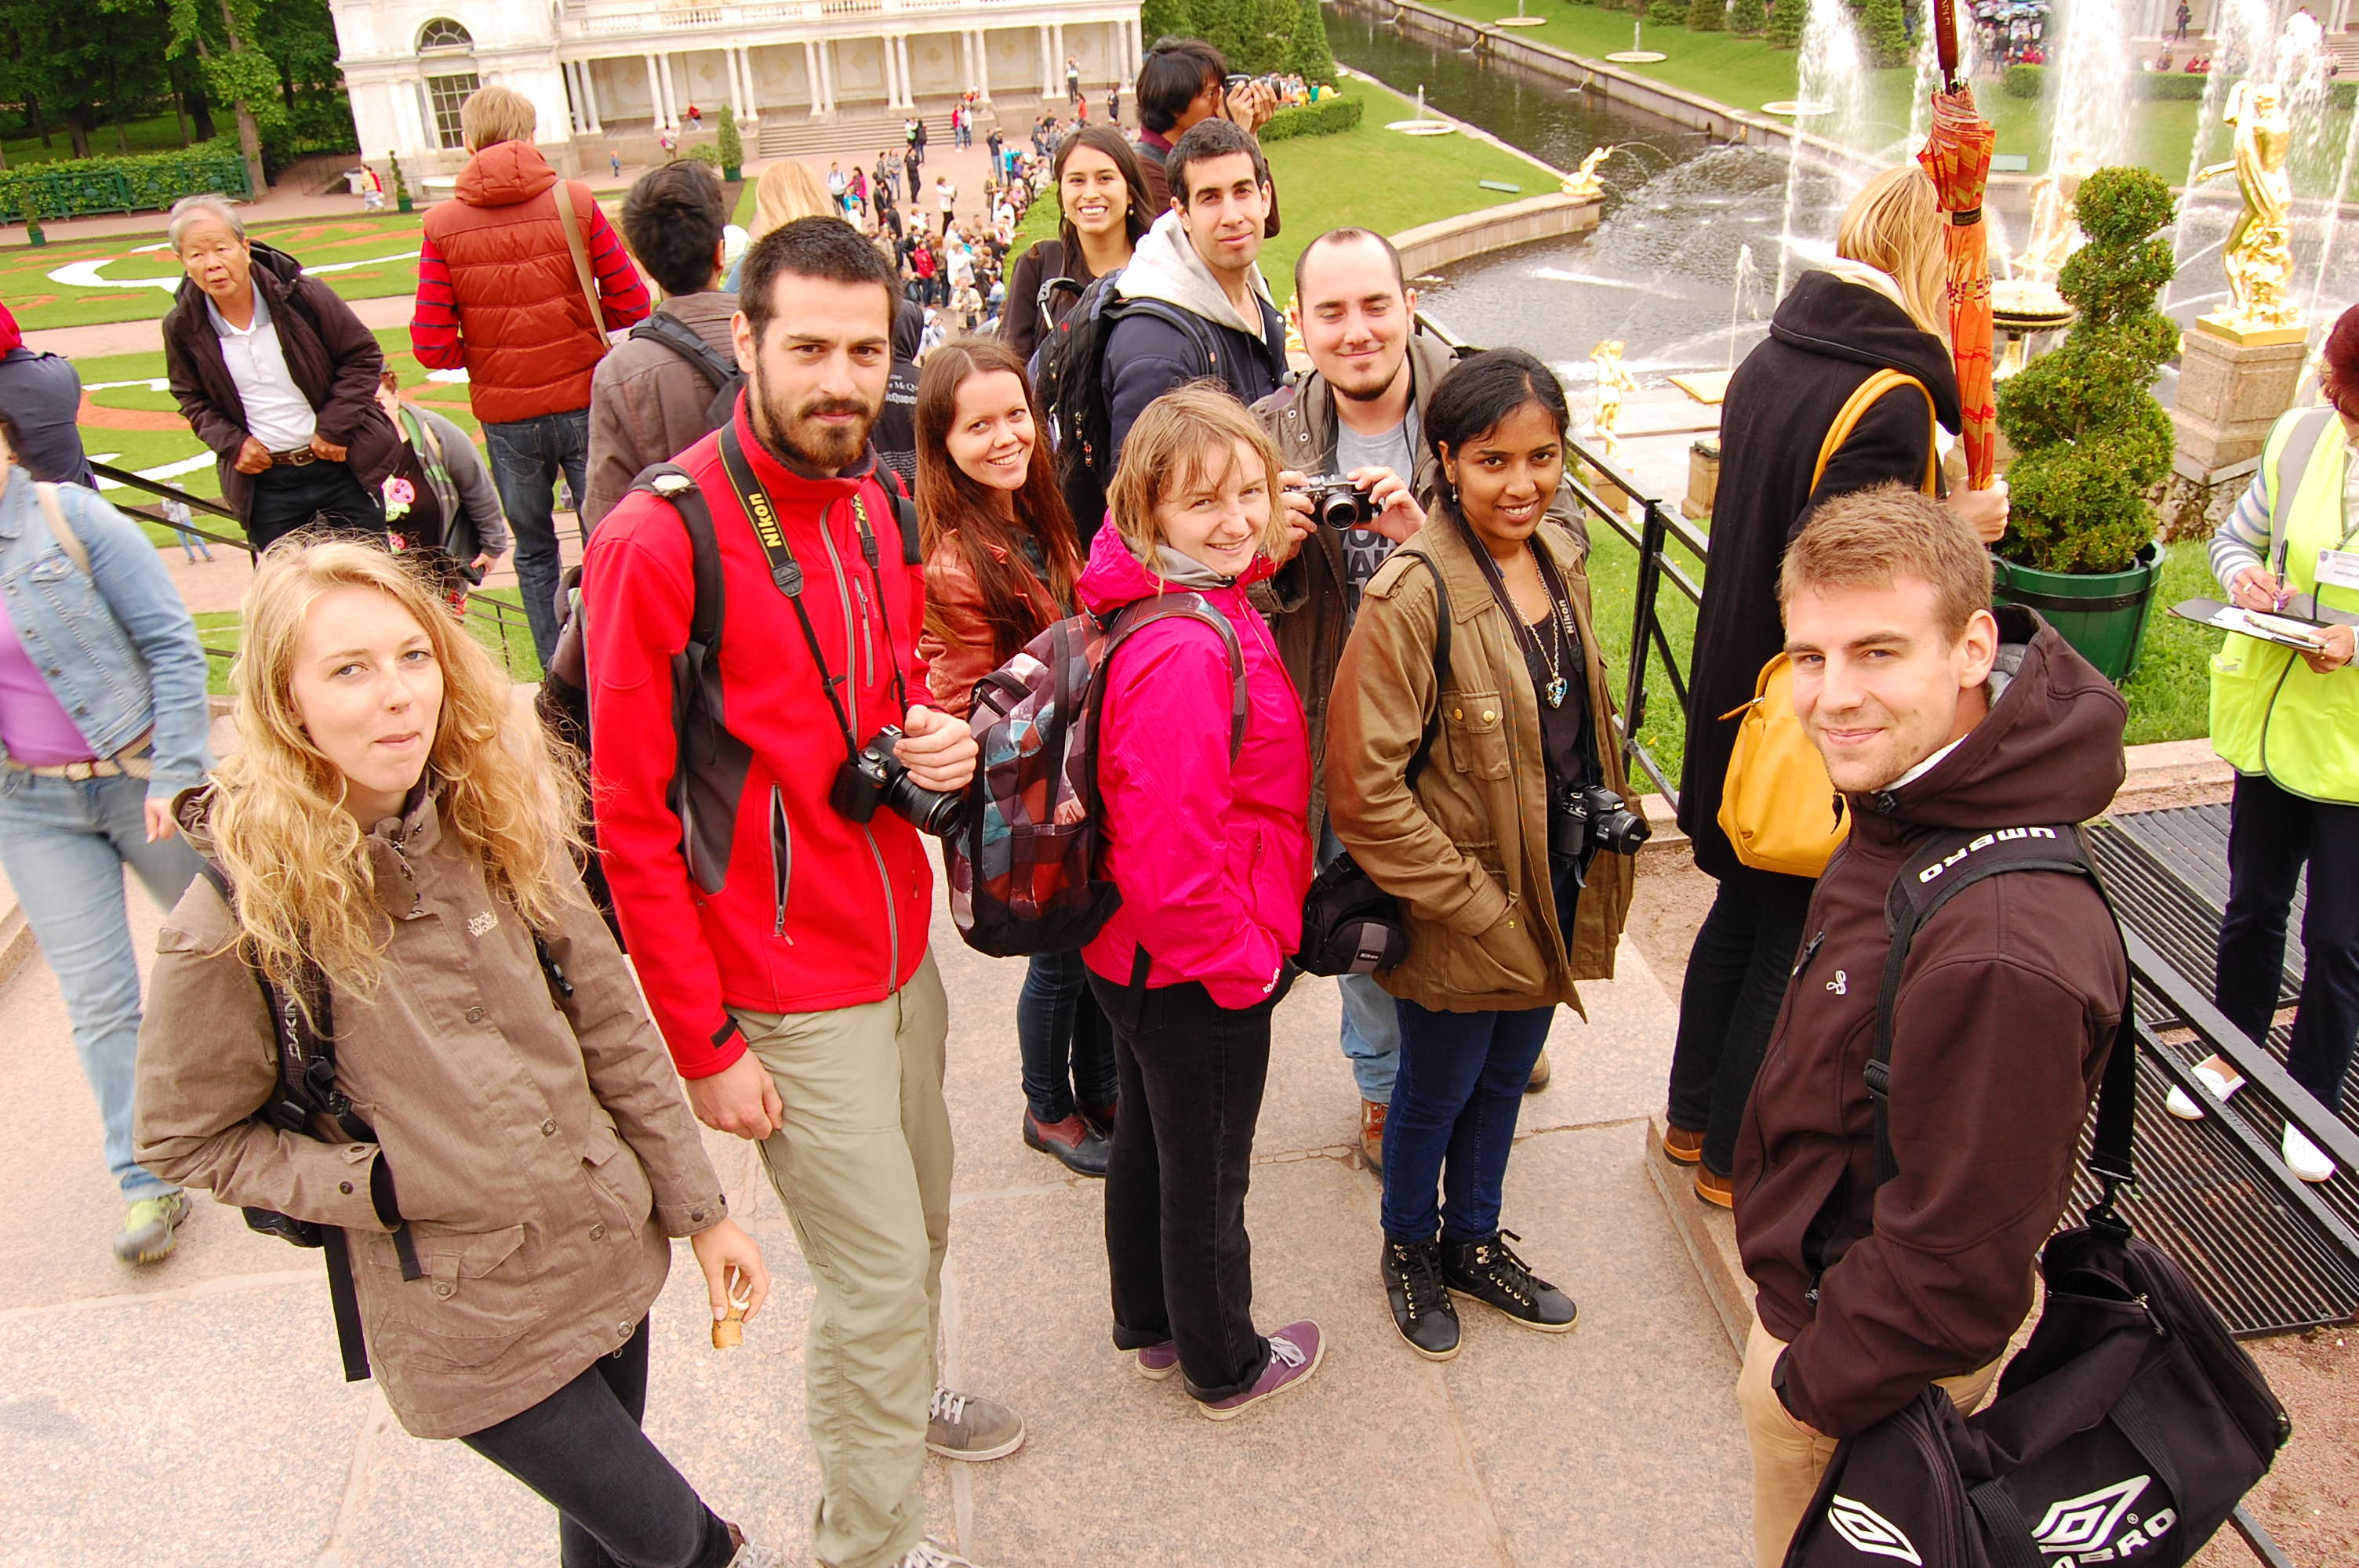
\includegraphics[width=0.38 \textwidth]{media/front_picture.jpg} \\
\end{wrapfigure}
	
\NewsItem{Author's thoughts} % Main next item title
\vspace{3pt} % Some extra whitespace since there is no author as for the news in the body of the newsletter
\textit{
%12345678901234567890123456789012345678901234567890123456789012345678901234567890
As a PhD student, we are often call to perform research studies and publish our
results in international conferences that take place in different parts of the world
as a payback for the hard effort you put in your work.
Such opportunity allows researchers to travel to conferences while their
affiliated institute pays for the flight, accommodation, and food expenses. 
Therefore, I had the luck to travel to many new different destinations
and explore places that I had no clue of them.
Moreover, anytime I was traveling, I always took advantage of such chances
to visit nearby countries of friends.
Eventually, while growing old and start lacking energy to travel or do various activities,
I take every change that I have to do alongside my work because when the time comes
I will have many great stories to share and laugh about!
}
\par\hfill --- Stefanos Georgiou
\end{minipage}
\end{center}

\vspace{0.5cm}
\SepRule % Small horizontal rule after the main news item
\vspace{0.5cm}

%\setlength{\columnsep}{16pt} % Uncomment to manually change the white space between columns
\begin{multicols}{3} % Begin the three-column layout

%----------------------------------------------------------------------------------------
%	OTHER NEWS
%----------------------------------------------------------------------------------------

\NewsItem{How it all started?}
Being at the second year of my PhD studies, it means I cab be in a position to write
and publish research articles to top-tier computer science conferences that more of the time
have acceptance rate close to 30\% of the submitted studies.
Therefore, during the September of 2017, I was constantly working a research study
to be submitted by the end of January 2018.
Along the many reasons I wanted to go the specific conference apart of being the most
prestigious in our field of studies, it was taking place in Gothenburg of Sweden.
Therefore, I could have the opportunity to visit my best friend Fisayo with whom I was
studying during my Masters, to visit Saint-Petersburg when I spend a whole semester
during my Masters and see my old friends there, and after to end up in Lappeenranta
of Finland to a summer school organized by my Master program.

All the above trips could be possible only if I could get my work accepted at the conference
and having some expenses covered from my institute and by the end of February I had my answer.
I was going to spend whole three weeks traveling to the above countries that I mentioned.
Moreover, after I inform the lab in Saint-Petersburg, where I did my Masters, they where
happy to invite me to present my research work there and give tutorial to Master students
regarding cutting-edge technologies that are currently used in the industry of software development.
Also, after informing the summer school that I could be there after my trip in Saint-Petersburg,
they invited me as a keynote speaker to present my work and views on the energy efficiency
of software development.

Being super happy about this, I immediately started planning my trip such as plane, bus, and
train tickets and accommodation.
Moreover, I had to issue a visa and go through again this painful process of collecting documents.
However, it was worthwhile just to visit again so many places where I had pleasant memories.


\NewsAuthor{Stefanos Georgiou}\begin{flushleft}
	
% Make discussion separated at four parts, one for each country of visit.
% Dicsuss on minor events too, such as strange things that happened
% or scafoldings done to gain further information regarding persons of interest.



\end{flushleft}

%-----------------------------------------------------------

\NewsItem{Gothenburg, Conference Time}
% Discuss about the attack you received from a group of blondies :)

\end{multicols} % End the three-column layout for a large picture

\begin{center}
\vspace{10pt}
	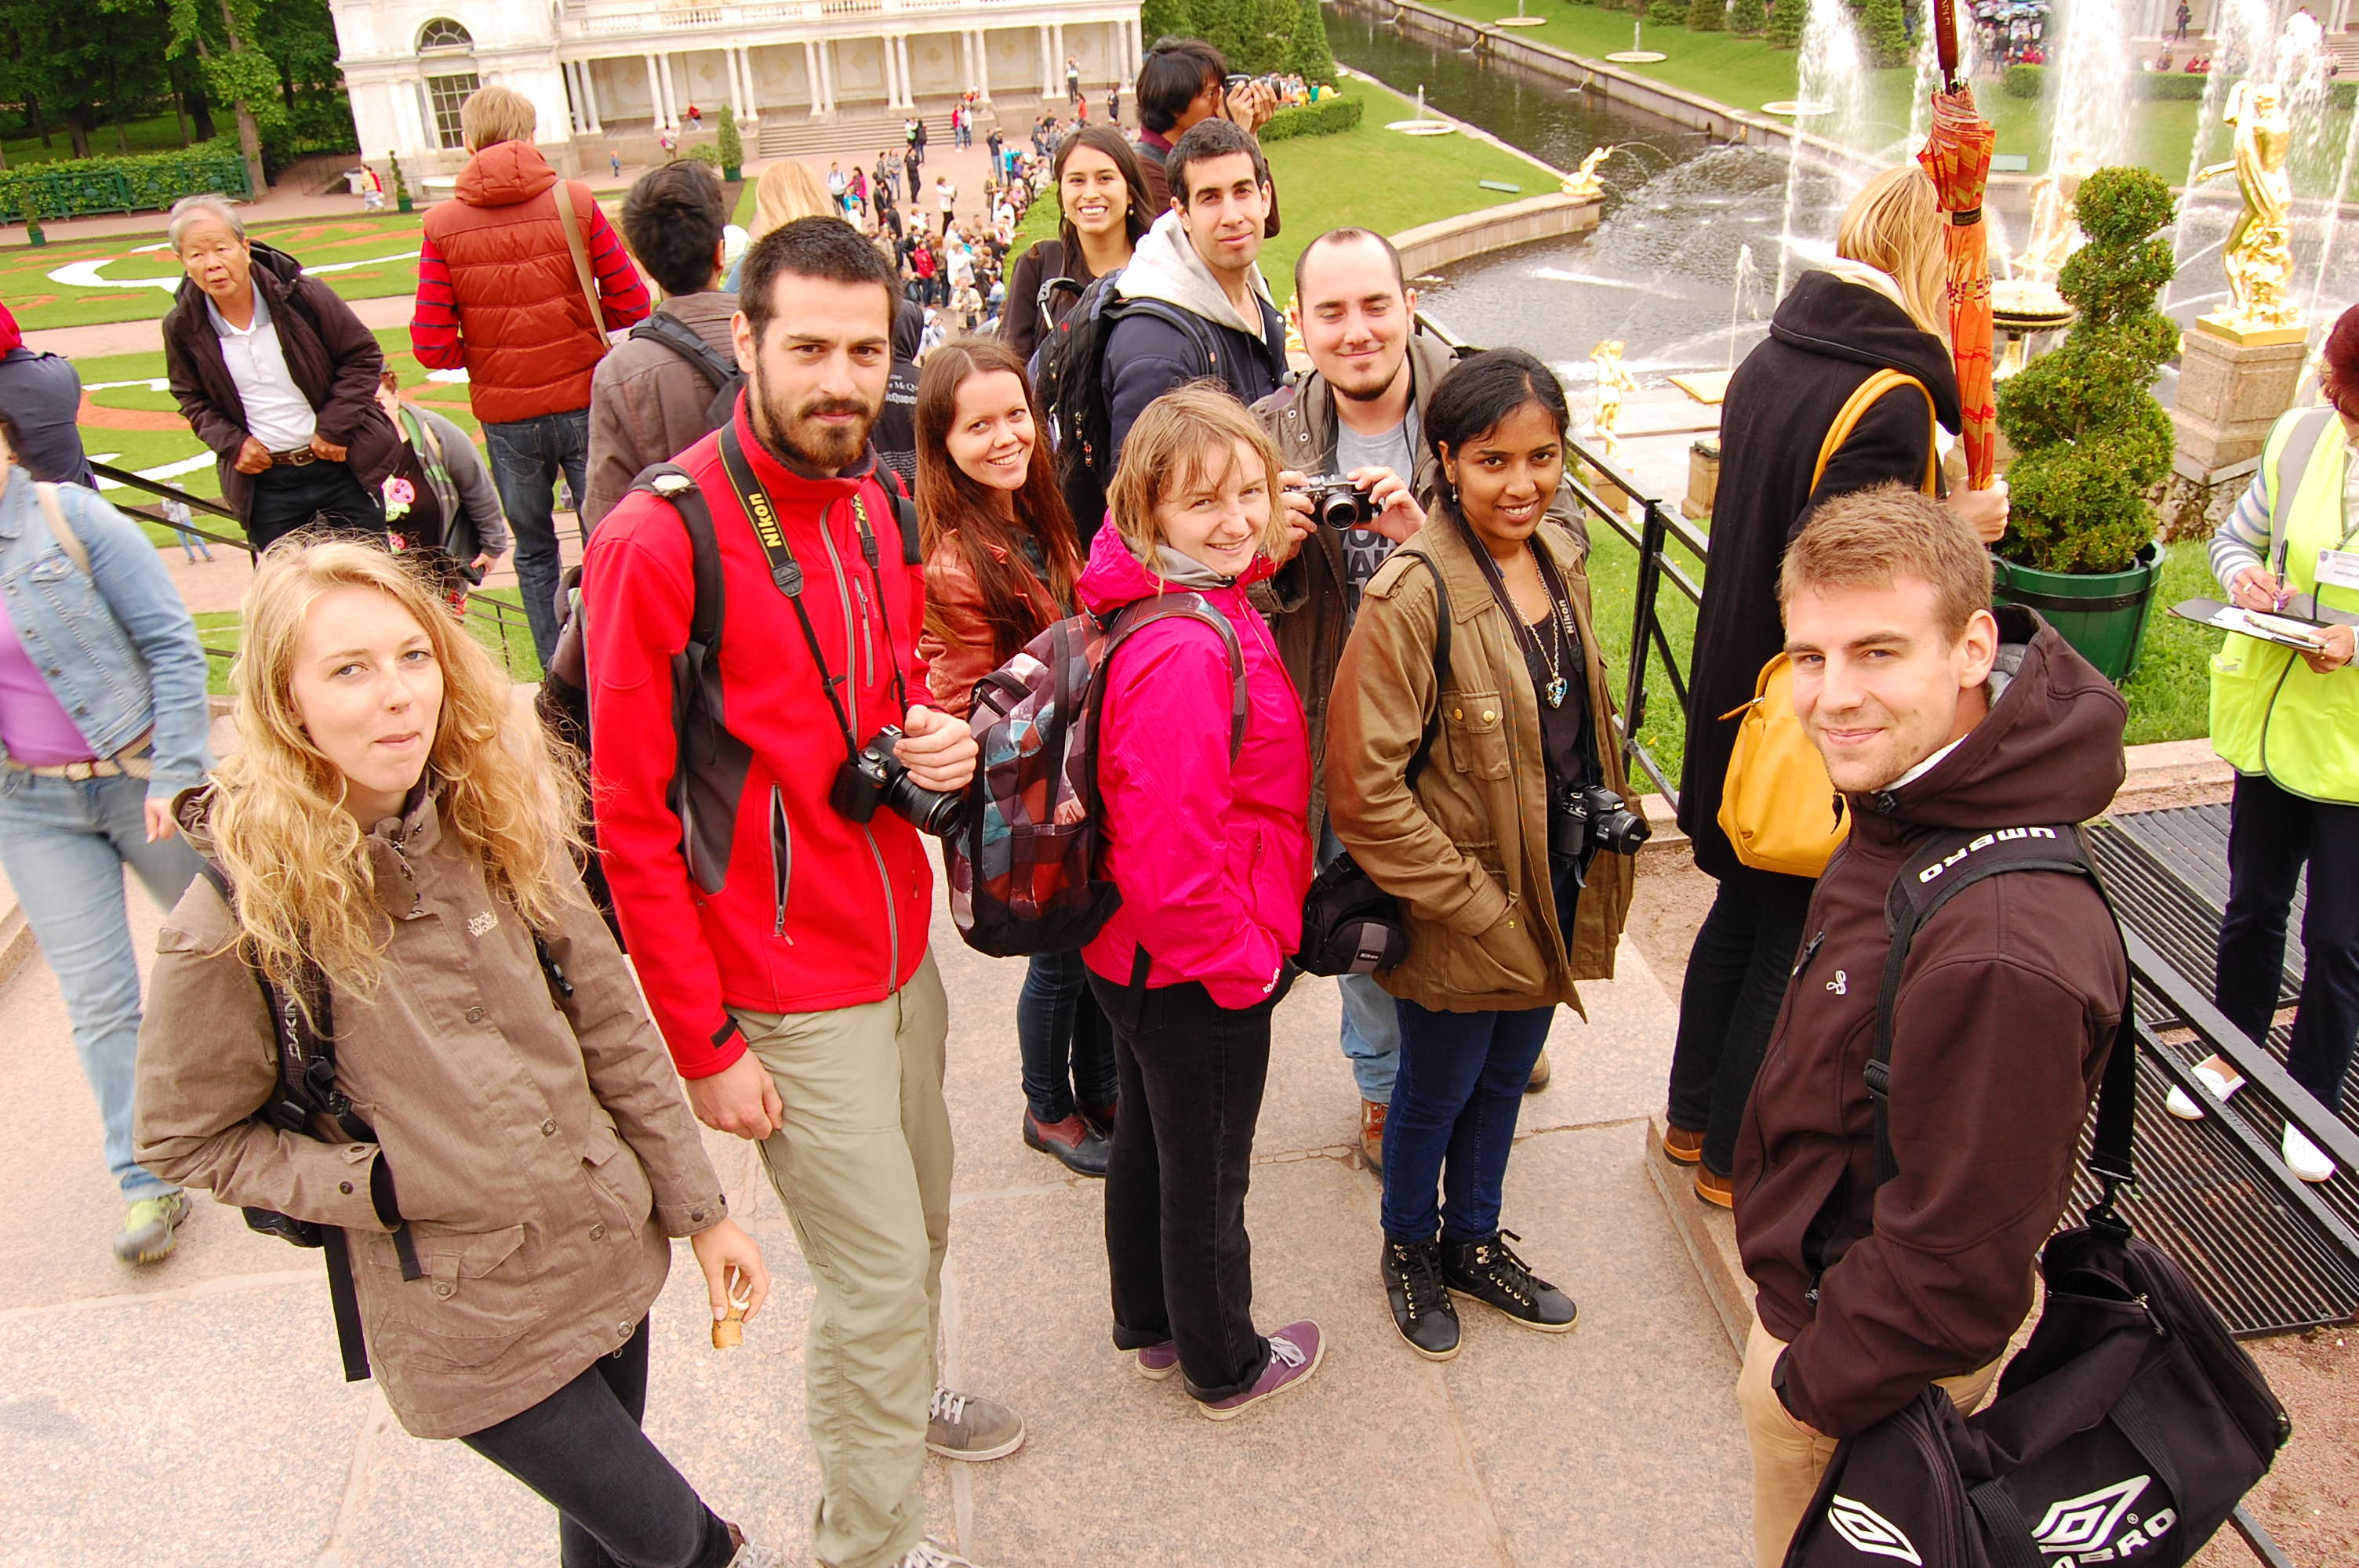
\includegraphics[width=0.8\linewidth]{media/front_picture.jpg}
	\\
\par\large\textit{Something something\ldots}
\vspace{10pt}
\end{center}

\begin{multicols}{3} % Continue the three-column layout

%-----------------------------------------------------------
\NewsItem{Copenhangen, Walking Time}

% Discuss about the missed trips and connected in with Fisayo's wedding.

%-----------------------------------------------------------
\NewsItem{Saint-Petersburg, Fun Time}


%-----------------------------------------------------------
\NewsItem{Lappeenranta, Summer School Time}

	
%-----------------------------------------------------------
\NewsItem{Take Home}


%-----------------------------------------------------------
\NewsItem{Acknowledgements}
	
	
\begin{quotation} % Example of a quotation
\noindent{\Huge``}

\noindent\normalsize\textit{
	Something something here too, still don't know what!
}

\hfill{\Huge''}

\end{quotation}

\NewsItem{Acknowledgments}

\end{multicols}

%----------------------------------------------------------------------------------------

\end{document} 
